\section{Game Overview}
In this section we will briefly talk about the game in which we implemented Neural Networks and Genetic Algorithms.
We made a significant number of changes from Assignment 1 to the extent that it is now a completely different game. 
Therefore, instead of emphasising each alteration, we will explain the new game rules as a whole.
In Assignment 2, you control the group
of flies and must search the map for resource trees. The resource trees are the apple tree (red) and flower tree (white).
The location of these trees is procedurally generated using a Genetic Algorithm at the beginning of the game. At a resource tree, the fly will begin to accumulate points which it must return to the "home tree" in order to increase the players score. For every 100 points scored, a fly will spawn.
The player has limited vision from
the light each fly emits, however, at random intervals lightning will strike revealing the maps objects as can be seen in Figure \ref{fig:lightning_compare}. During the course
of the game, the player must also be cautious of the frog predator which eats their flies. The frog is implemented using Neuroevolution, in particular, Genetic Algorithms and Neural Networks.
\begin{figure}[h]
        \centering
        \begin{subfigure}[b]{0.492\linewidth}
                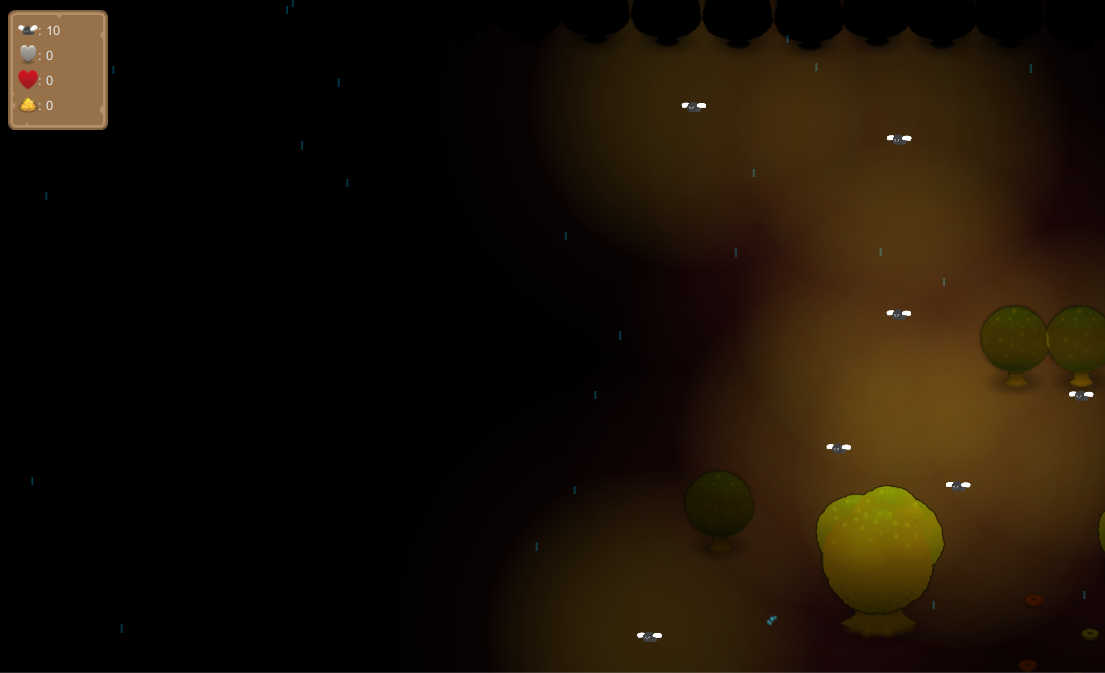
\includegraphics[width=\linewidth]{./no_lightning}
                \caption{The lighting in the scene when there is no lightning.}
                \label{fig:lightning}
        \end{subfigure}
        \begin{subfigure}[b]{0.49\linewidth}
                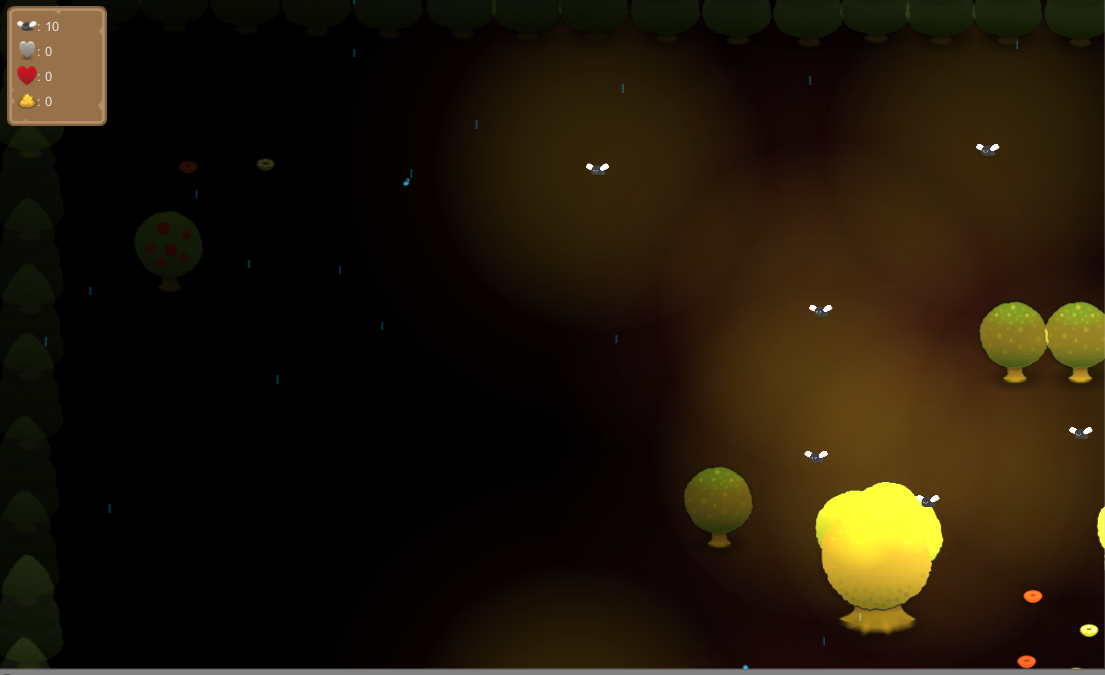
\includegraphics[width=\linewidth]{./lightning}
                \caption{The lighting in the scene when lightning strikes.}
                \label{fig:no_lightning}
        \end{subfigure}
        \caption{The effects of lightning on the scene.}
        \label{fig:lightning_compare}
\end{figure}

\section{Objectives}
For this project we had the following core objectives:
\begin{itemize}
\item Implement Genetic Algorithms and Neural Networks in a game environment as a learning exercise. Neither of
us had applied either algorithm before and we were both interested in learning them.
\item Use a Genetic Algorithm to procedurally place trees on the map to add variation for the player
and enhance overall gameplay.
\item Use a Genetic Algorithm to evolve a Neural Network which controls the steering of a frog agent which
acts as the players adversary.
\end{itemize}